% !TEX root = ../main.tex

% 报告主体


%---------------------------------------------------------------------
% 实验
\clearpage
\JMSection{实验}


\subsection{实验系统搭建}

本实验根据几何光学成像原理搭建光路系统,具体步骤如下:

\begin{enumerate}
    \item \textbf{器件安装与距离设置}
    将绿光 LED、镂空板、镜头、相机依照几何光学成像装置的基本结构安装在面包板上。
    \begin{itemize}
        \item LED 与镂空板间距为 \SI{38.5}{cm}
        \item 镜头前端距离镂空板为 \SI{68}{cm}
        \item 镜头光圈设置为 F5.6,焦距约为 \SI{70}{mm}
    \end{itemize}

    \item \textbf{成像调焦与散斑引入}
    \begin{itemize}
        \item 移除散射片,设置镜头光圈为 F5.6,并调节视场至最小(即放大率最大)
        \item 关闭 LED 光源,调节镜头对焦环,使显示屏中的字母清晰成像
        \item 打开 LED 光源,插入 \SI{1}{\degree}散射片
    \end{itemize}

    \item \textbf{调节放大率}
    调节镜头的放大率环,使字母图像刚好被散斑覆盖。
    \textbf{完成此步骤后,LED、镂空板、镜头和相机的位置不再调整},系统搭建完成。
\end{enumerate}



\subsection{数据处理原理}


  \begin{figure}[H]
    \begin{minipage}[b]{0.48\linewidth}
      \centering
      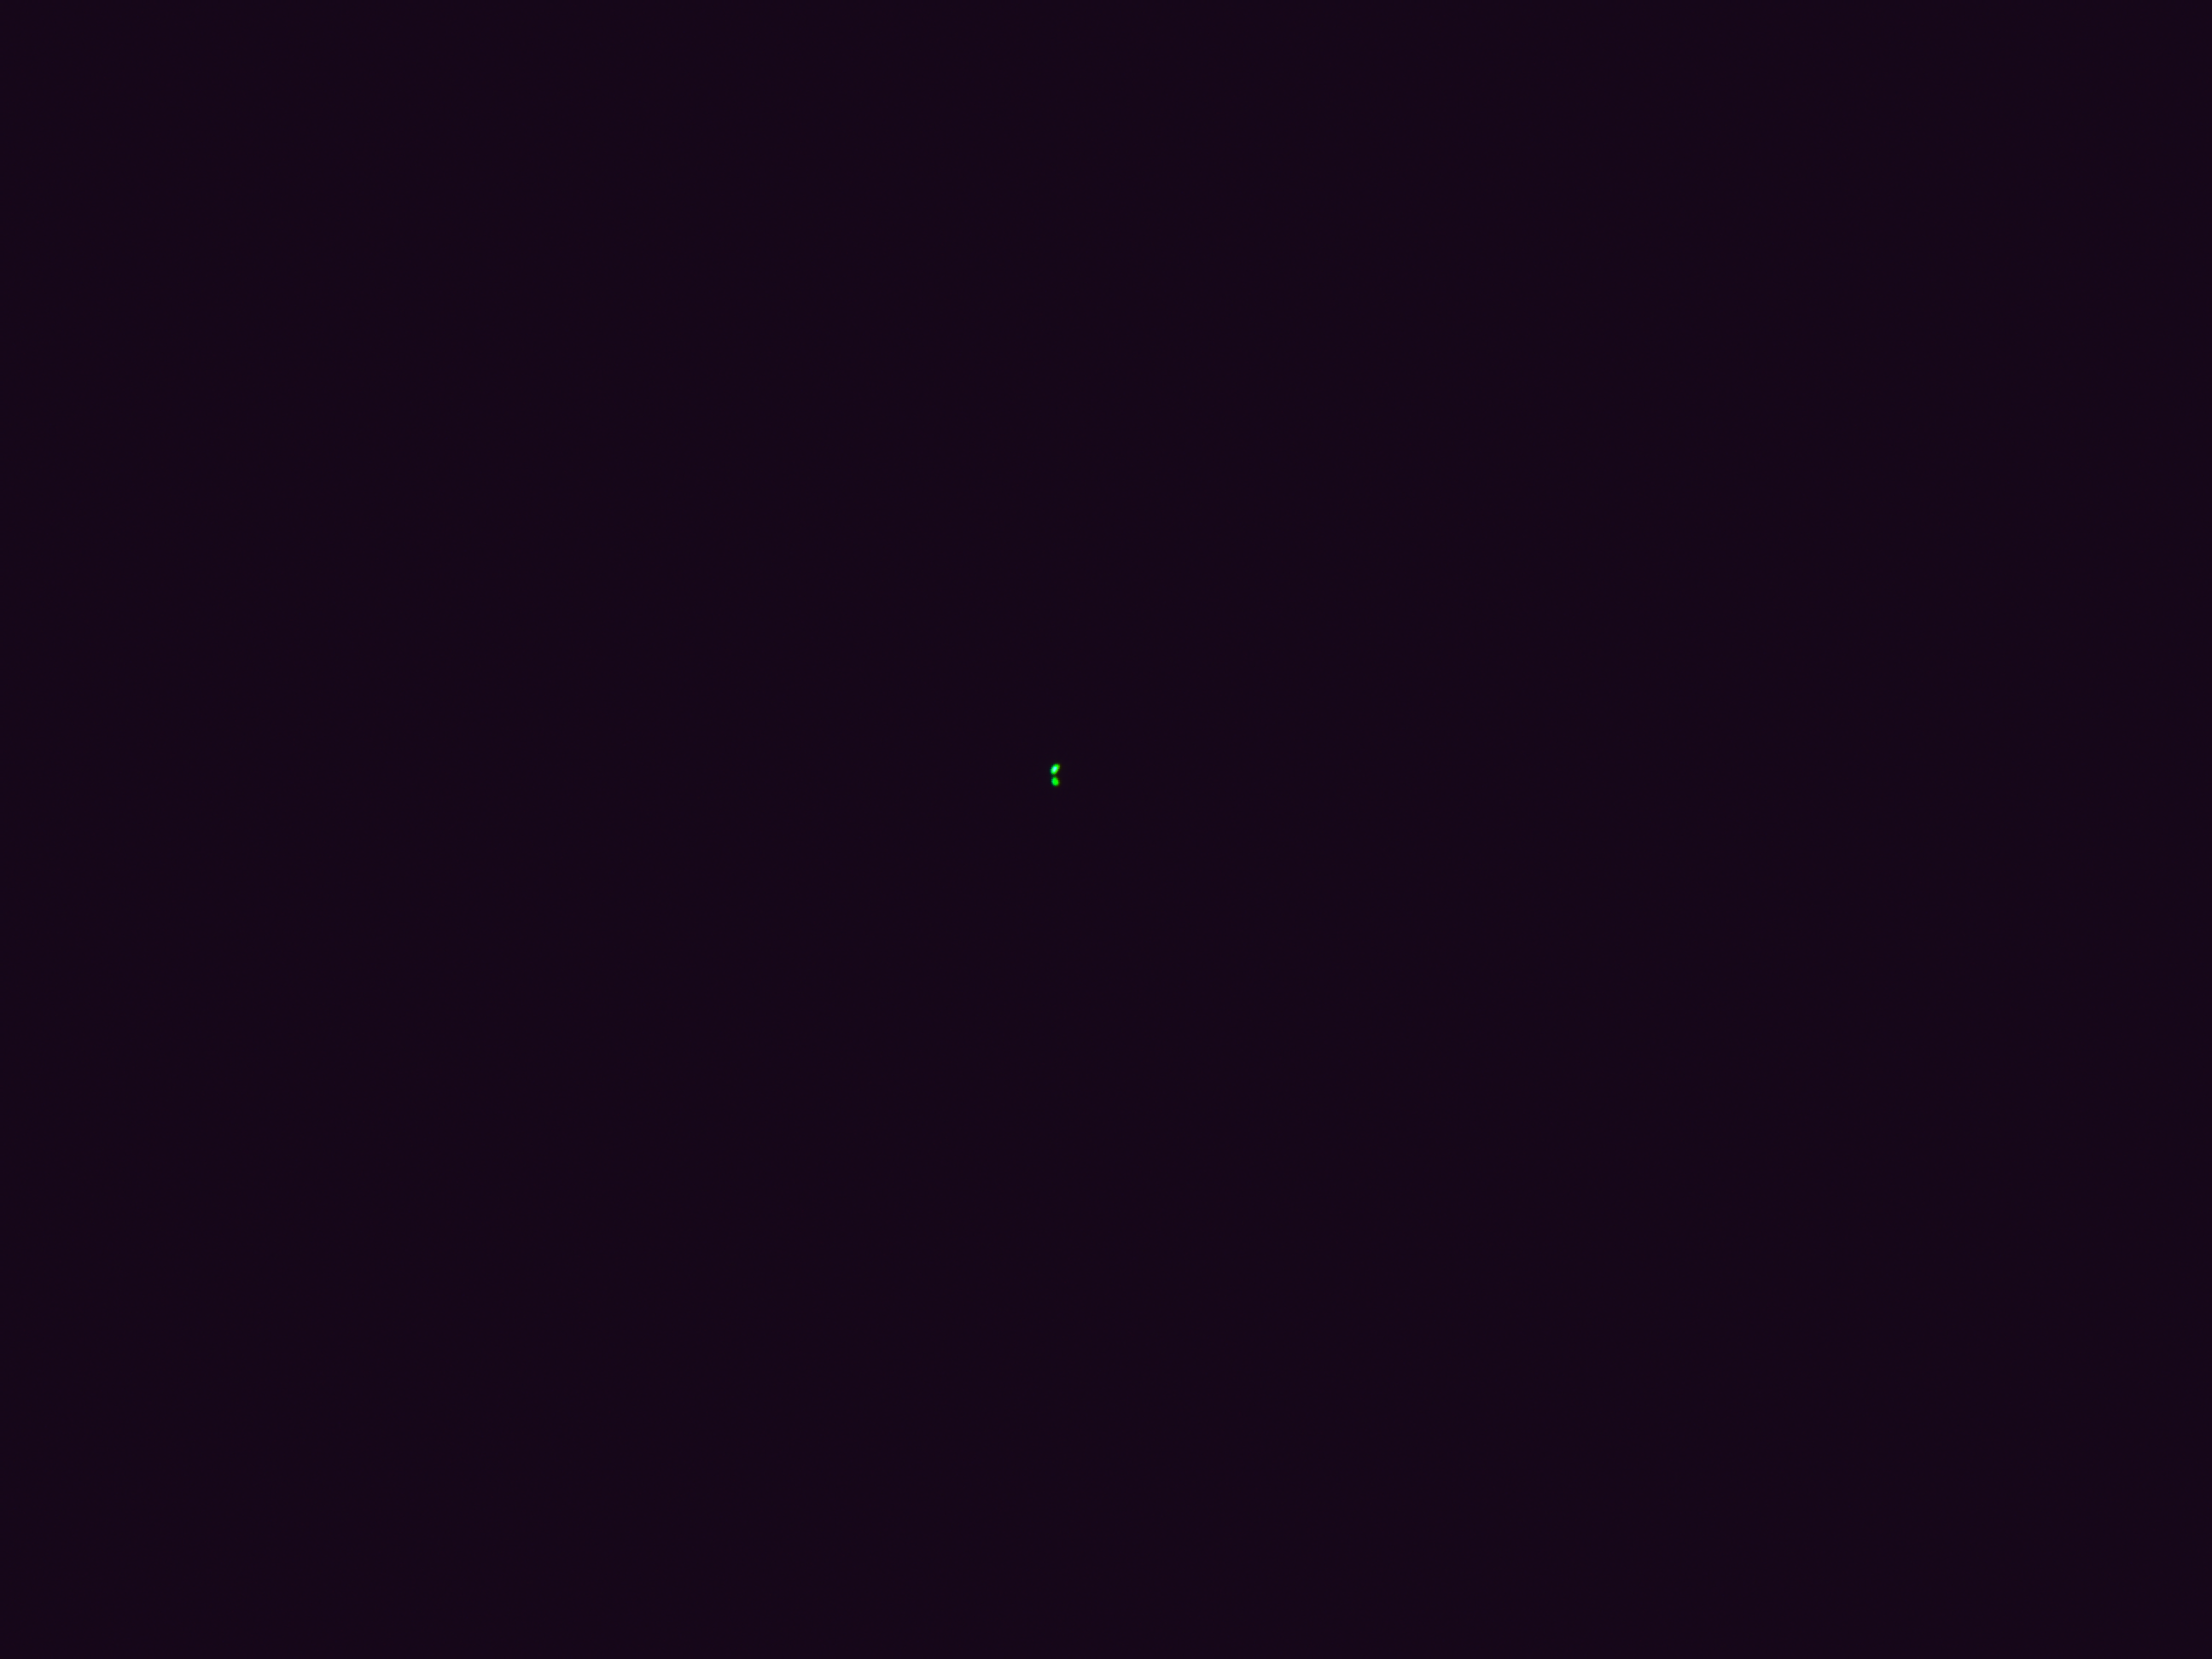
\includegraphics[width=\linewidth]{实验一/分析/参考物.png}
      \caption{参考物}
      \label{fig:点扩散函数参考物}
    \end{minipage}
    \hfill
    \begin{minipage}[b]{0.48\linewidth}
      \centering
      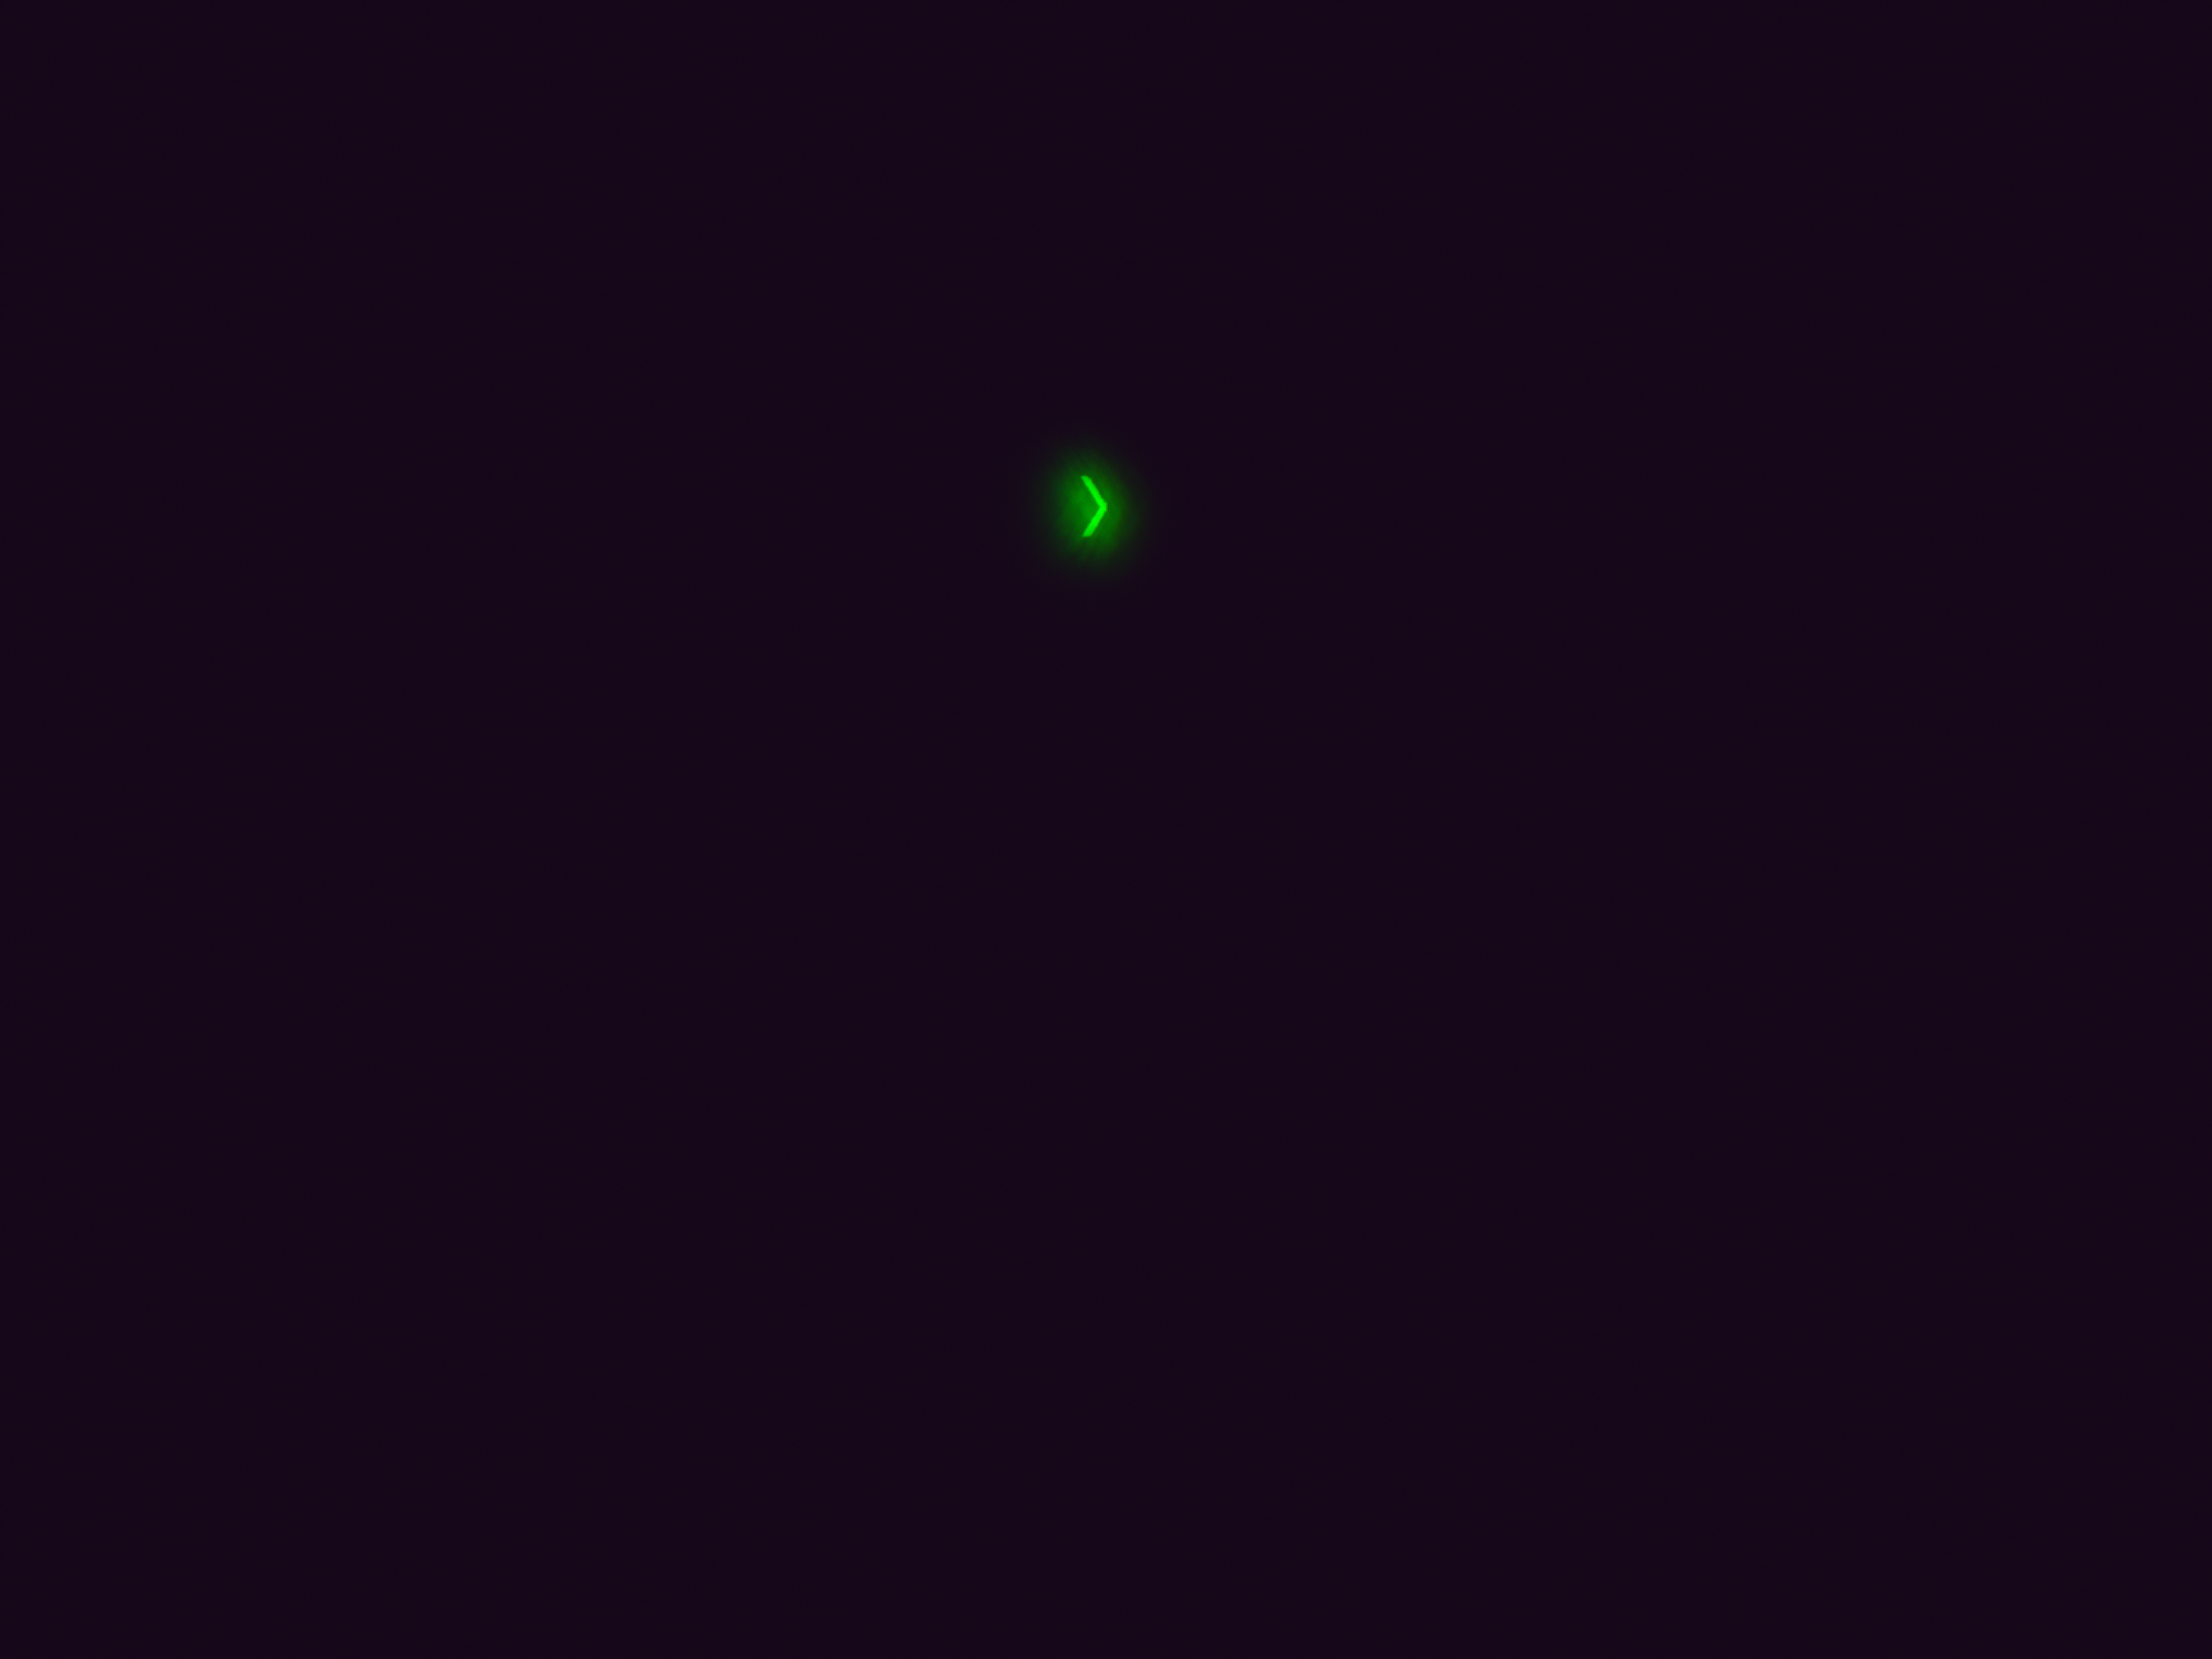
\includegraphics[width=\linewidth]{images/实验一/分析/参考散斑}
      \caption{参考散斑}
      \label{fig:点扩散函数参考散斑}
    \end{minipage}
  \end{figure}
  \begin{figure}[{H}]
    \centering
    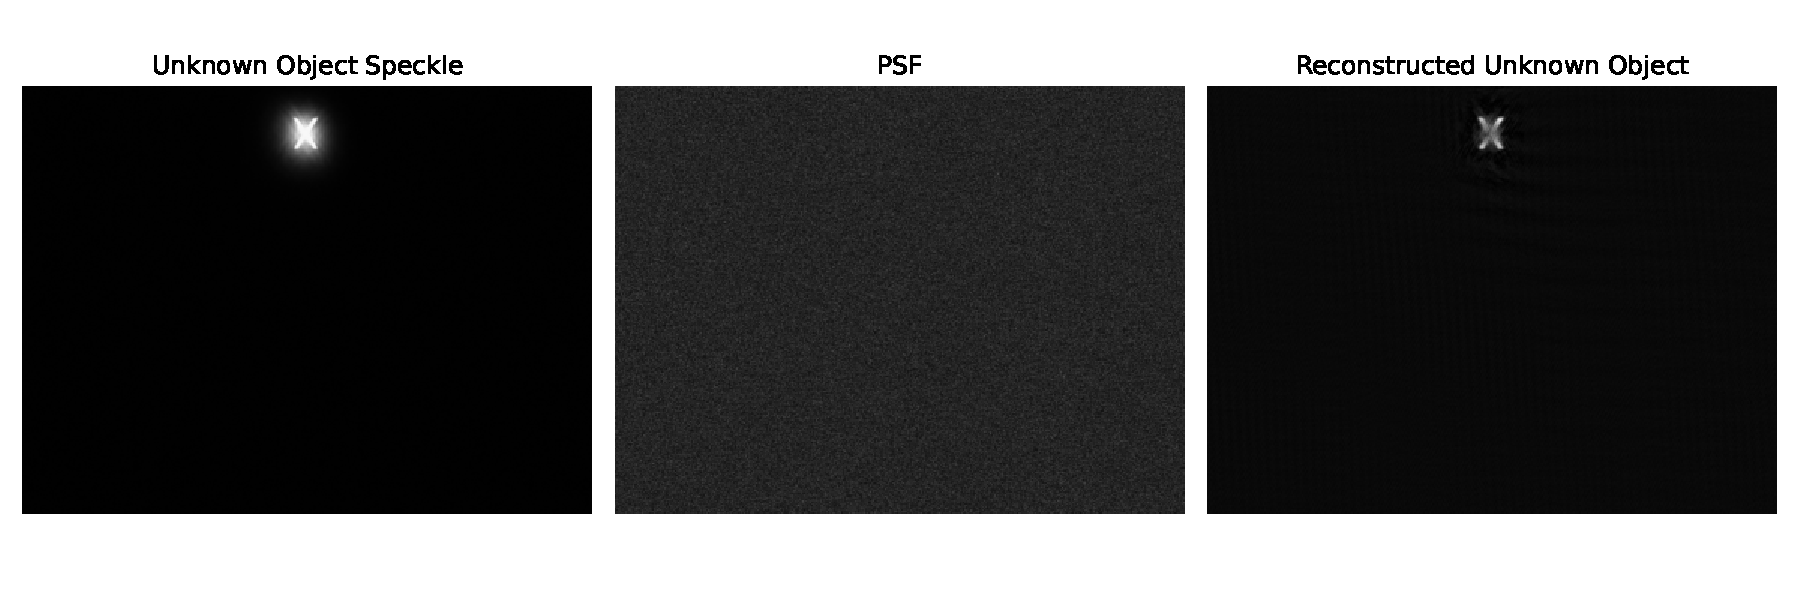
\includegraphics[width=0.8\linewidth]{images/实验一/分析/图像对比图.pdf}
    \caption{图像对比图}
    \label{fig:点扩散函数图像重建}
  \end{figure}




  我们首先将字母遮挡一半,作为参考物(\cref{fig:点扩散函数参考物})和参考散斑(\cref{fig:点扩散函数参考散斑}),用于求解点扩散函数;随后去掉遮挡,作为我们的未知物散斑,并使用刚刚求解的点扩散函数进行图像重建(\cref{fig:点扩散函数图像重建})。

  



\subsection{记忆效应范围测量}

  


  \begin{figure}[H]
      \centering
      \includegraphics[width=0.8\linewidth]{实验一/-4mm/image_comparison.pdf}
      \caption{-4mm图像对比图}
      \label{fig:-4mm图像对比图}
  \end{figure}


  \begin{figure}[H]
      \centering
      \includegraphics[width=0.8\linewidth]{实验一/-3mm/image_comparison.pdf}
      \caption{-3mm图像对比图}
      \label{fig:-3mm图像对比图}
  \end{figure}


  \begin{figure}[H]
      \centering
      \includegraphics[width=0.8\linewidth]{实验一/-2mm/image_comparison.pdf}
      \caption{-2mm图像对比图}
      \label{fig:-2mm图像对比图}
  \end{figure}


  \begin{figure}[H]
      \centering
      \includegraphics[width=0.8\linewidth]{实验一/-1mm/image_comparison.pdf}
      \caption{-1mm图像对比图}
      \label{fig:-1mm图像对比图}
  \end{figure}


  \begin{figure}[H]
      \centering
      \includegraphics[width=0.8\linewidth]{实验一/0mm/image_comparison.pdf}
      \caption{0mm图像对比图}
      \label{fig:0mm图像对比图}
  \end{figure}


  \begin{figure}[H]
      \centering
      \includegraphics[width=0.8\linewidth]{实验一/+1mm/image_comparison.pdf}
      \caption{+1mm图像对比图}
      \label{fig:+1mm图像对比图}
  \end{figure}


  \begin{figure}[H]
      \centering
      \includegraphics[width=0.8\linewidth]{实验一/+2mm/image_comparison.pdf}
      \caption{+2mm图像对比图}
      \label{fig:+2mm图像对比图}
  \end{figure}


  \begin{figure}[H]
      \centering
      \includegraphics[width=0.8\linewidth]{实验一/+3mm/image_comparison.pdf}
      \caption{+3mm图像对比图}
      \label{fig:+3mm图像对比图}
  \end{figure}

  \begin{figure}[H]
      \centering
      \includegraphics[width=0.8\linewidth]{实验一/+4mm/image_comparison.pdf}
      \caption{+4mm图像对比图}
      \label{fig:+4mm图像对比图}
  \end{figure}


  在记忆效应范围测量实验中,我们将字母板左右平移,分别测量不同位置的散斑,并使用\textbf{未平移}时所求解的点扩散函数进行图像重建,结果如(\cref{fig:-4mm图像对比图}--\cref{fig:+4mm图像对比图})所示。

  观察重建图像的效果可知,在平移范围在 ($\Delta x \in (-1, +3) $mm)内,图像重建效果均较好,说明该光学系统的记忆效应范围大约为($\pm 2$mm)。

  但是我们发现,该记忆效应范围区间没有关于 0 对称,这是因为我们的字母在 “0mm” 位置时并不在光轴上。

% 对于记忆效应的测量,观察图像可知,在1mm范围内,可以观察到恢复图像的效果较好,在1mm之外就会出现无法分辨出原始字母的情况,可以认定为:记忆效应的范围为1mm。




\subsection{实验二:散射光成像的影响条件}

\subsubsection{旋转记忆效应}
% ============ 旋转记忆效应 ============
  % 大角度旋转
  \begin{figure}[H]
      \centering
      \includegraphics[width=0.8\linewidth]{实验二/旋转记忆效应/大角度旋转/图像对比图.pdf}
      \caption{大角度旋转图像对比图}
  \end{figure}

  % 小角度旋转
  \begin{figure}[H]
      \centering
      \includegraphics[width=0.8\linewidth]{实验二/旋转记忆效应/小角度旋转/图像对比图.pdf}
      \caption{小角度旋转图像对比图}
  \end{figure}

  旋转记忆效应是指当散射片绕垂直于光传播方向的轴发生微小旋转时,出射散斑图不会完全改变,而是整体发生旋转,保持一定的空间相关性。在实验中轻轻旋转散射片时图像仍能重建,说明系统处于旋转记忆效应有效范围内;但若旋转角度过大,相关性丧失,重建将失败。因此,适度旋转下的成像稳定性体现了散射系统的旋转记忆能力。

  根据实验结果来看,小角度和大角度均可以分辨出图像,但是从效果上来看,小角度的成像效果是优于大角度的。






\subsubsection{焦距的影响}
% ============ 焦距的影响 ============
  % 工作距离50 - 焦距18mm
  \begin{figure}[H]
      \centering
      \includegraphics[width=0.8\linewidth]{实验二/焦距的影响/工作距离50/焦距18/图像对比图.pdf}
      \caption{工作距离50cm-焦距18mm图像对比图}
  \end{figure}

  % 工作距离50 - 焦距40mm
  \begin{figure}[H]
      \centering
      \includegraphics[width=0.8\linewidth]{实验二/焦距的影响/工作距离50/焦距40/图像对比图.pdf}
      \caption{工作距离50cm-焦距40mm图像对比图}
  \end{figure}

  % 工作距离50 - 焦距108mm
  \begin{figure}[H]
      \centering
      \includegraphics[width=0.8\linewidth]{实验二/焦距的影响/工作距离50/焦距108/图像对比图.pdf}
      \caption{工作距离50cm-焦距108mm图像对比图}
  \end{figure}

  % 工作距离68cm - 焦距18mm
  \begin{figure}[H]
      \centering
      \includegraphics[width=0.8\linewidth]{实验二/焦距的影响/工作距离68/焦距18/图像对比图.pdf}
      \caption{工作距离68cm-焦距18mm图像对比图}
  \end{figure}

  % 工作距离68cm - 焦距40mm
  \begin{figure}[H]
      \centering
      \includegraphics[width=0.8\linewidth]{实验二/焦距的影响/工作距离68/焦距40/图像对比图.pdf}
      \caption{工作距离68cm-焦距40mm图像对比图}
  \end{figure}

  % 工作距离68cm - 焦距108mm
  \begin{figure}[H]
      \centering
      \includegraphics[width=0.8\linewidth]{实验二/焦距的影响/工作距离68/焦距108/图像对比图.pdf}
      \caption{工作距离68cm-焦距108mm图像对比图}
  \end{figure}


  镜头焦距决定了成像系统的放大倍率和视场大小,从而影响对散斑图的采集能力。在散射光成像中,较短焦距提供较大的视场和更高的光通量,有助于获取完整的散斑图结构,但角度分辨率较低,不利于微小扰动下的成像重建;而较长焦距则提高了角度分辨率和对细节的敏感性,使记忆效应下散斑图的微小位移更加明显,有利于图像恢复,但光强降低、视场变小,对系统稳定性要求更高。因此,焦距的选择需在视场范围、分辨能力与信噪比之间权衡,以获得最佳重建效果。

  观察我们的数据可知,我们选择不同的焦距均没有成功重建图像,主要是因为在改变不同实验条件时,没有调整为共轴。







  
\subsubsection{工作距离}
% ============ 工作距离的影响 ============

  \begin{itemize}
    \item 第一次实验

      % 工作距离50cm
      \begin{figure}[H]
          \centering
          \includegraphics[width=0.8\linewidth]{实验二/工作距离的影响/工作距离50cm/图像对比图.pdf}
          \caption{工作距离50cm图像对比图}
      \end{figure}

      % 工作距离60cm
      \begin{figure}[H]
          \centering
          \includegraphics[width=0.8\linewidth]{实验二/工作距离的影响/工作距离60cm/图像对比图.pdf}
          \caption{工作距离60cm图像对比图}
      \end{figure}
      根据实验图像来看,均无明显的较好效果。分析原因后,我们发现主要是两个原因导致重建失败,一个是“图像过曝”,导致高频的信息缺失;一个是整个光路未对齐,导致出现像差,使得散斑所携带的信息被识别成了噪声。
      
      之后我们重新调整了光路,重新测量了这部分实验内容,见后。

    \item 第二次实验

      \begin{figure}[H]
          \centering
          \includegraphics[width=0.8\linewidth]{二次实验/50cm_2/图像对比图.pdf}
          \caption{工作距离50cm图像对比图}
      \end{figure}

      \begin{figure}[H]
          \centering
          \includegraphics[width=0.8\linewidth]{二次实验/55cm_2/图像对比图.pdf}
          \caption{工作距离55cm图像对比图}
      \end{figure}
      \begin{figure}[H]
          \centering
          \includegraphics[width=0.8\linewidth]{二次实验/60cm_2/图像对比图.pdf}
          \caption{工作距离60cm图像对比图}
      \end{figure}
 
      % 观察可以发现,工作距离越长,成像效果变差了一点,但是具体来看,在这个实验条件下,可能的确影响不大。    
      理论上,工作距离决定了系统对散斑图的角度分辨能力和信噪比,从而显著影响图像重建效果。距离过短时,角度扰动引起的散斑位移不明显,难以利用记忆效应重建图像;而距离过长虽可放大角度响应,有利于记忆效应的利用,但信号衰减严重,噪声上升,系统更易受干扰。因此,应在角度灵敏度与信噪比之间取得平衡,选择适中的工作距离以获得最佳重建效果。

      由我们的实验结果可知,在我们的实验条件下,工作距离范围较大,在($L \in (50, 60)$cm)的范围内均能够重建图像。




    \end{itemize}
  




\subsubsection{不同散射片}
% ============ 不同散射片 ============
  % 0.5° 散射片
  \begin{figure}[H]
      \centering
      \includegraphics[width=0.8\linewidth]{实验二/不同散射片/0.5°/图像对比图.pdf}
      \caption{0.5°散射片图像对比图}
  \end{figure}

  % 5° 散射片
  \begin{figure}[H]
      \centering
      \includegraphics[width=0.8\linewidth]{实验二/不同散射片/5°/图像对比图.pdf}
      \caption{5°散射片图像对比图}
  \end{figure}

  % 10° 散射片
  \begin{figure}[H]
      \centering
      \includegraphics[width=0.8\linewidth]{实验二/不同散射片/10°/图像对比图.pdf}
      \caption{10°散射片图像对比图}
  \end{figure}

  % 同散射片,随着散射片角度的增大,成像效果越来越差。
  在本实验中,我们通过更换不同度数的散射片,探究不同条件对散射光成像的影响。

  可以看到,在实验一中,我们使用 1° 的散射片进行相关测量,能够成功重建图像;在此实验中,我们更换了 0.5°、5°、10° 的散射片,均不能成功重建图像。

  对于 5°、10° 两种散射片,其散射过强,入射光经过大量多次散射,路径混合,所以微小角度或位移改变不会导致出射场的规律性移动,而是完全重构,导致出射光场中不再保留可用于重建的信息;对于 0.5° 的散射片,我们认为其被过度使用导致其实际散射效果超过标称的 0.5°,导致重建失败。




\subsubsection{总结}

  本实验通过改变旋转角度、焦距、工作距离及散射片种类,分析了不同条件对散射光成像效果的影响。
  
  结果表明:轻微旋转散射片仍能保持较高的散斑相关性,图像可重建,体现了旋转记忆效应;适当焦距有助于平衡视场和角度分辨率,提升成像质量;合适的工作距离可增强角度扰动对散斑的响应,利于图像恢复;而散射角过大会破坏图像重建条件,1°散射片在保持足够散斑特征与空间相关性的同时,实现了较好的重建效果。


